\subsection{Order finding}
We present a quantum algorithm that, given $a$ and $n$ such that $a<n, \gcd(a,n)=1$ on input, finds $r$ such that $a ^r=1 \mod n$. In other words, it finds the order of $a$ in group $\mathbb{Z}_n^*$, it's corresponding quantum circuit is presented on figure \ref{fig:shor}.
\\\\
In the algorithm we use two quantum registers. first will hold the value $a^x \mod n$ and the second will store the exponent $x$, initially both registers are set to ground state. As we need to utilize QFT, the registers' lengths need to be powers of 2; $m=\lceil\log n\rceil$.\\\\
first we initialize the first register with $m$ Hadamard gates, so it is in superposition of all possible $x$ resulting in a state:
\begin{align*}
    \ket{\xi}=\frac{1}{\sqrt{m}}\sum_{x=0}^{m-1}\ket{x}\ket{1}
\end{align*}
then we compute the function $f(x)=a^x \: \text{mod}\: n$, and put the result in the second register resulting in:
\begin{align*}
    \ket{\xi}=\frac{1}{\sqrt{m}}\sum_{x=0}^{m-1}\ket{x}\ket{a^x\: \text{mod}\: n}
\end{align*}
then we measure the second register to get value $y_0$. as we know the value in the second register, value in the first register is restricted so that $a^x \mod{n}=y_0$. it can be thus written as $x_0+lr$, where $x_0$ is the smallest x sufficing the condition, the current state is then:
\begin{align*}
  \ket{\xi}=\frac{1}{\sqrt{\lceil m/r \rceil}}\sum_{l=0}^{\lceil m/r \rceil-1}\ket{x_0 + lr}\ket{y_0}
\end{align*}
then we apply QFT to the first register, to obtain the number $x$. 
\begin{align*}
  \ket{\xi}=\frac{1}{\sqrt{m}\sqrt{\lceil m/r \rceil}}\sum_{x=0}^m\sum_{l=0}^{\lceil m/r \rceil-1}\left[e^{2\pi i (x_0+lr)x/m}\ket{x}\right]\ket{y_0}
\end{align*}  
The probability of obtaining certain $x$ upon measurement is clearly proportional to $e^{2\pi (x_0+lr)x/m}$. from this we derive that probabilities will peak for values of $x$ close to $\frac{m}{r}$.
\begin{figure}[ht!]
    \centering
    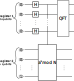
\includegraphics[width=0.65\linewidth]{30_licencjat/tex/figures/shor.png}
    \caption{Quantum circuit of order finding algorithm}
    \label{fig:shor}
\end{figure}
\newpage
We measure the value on the first register, resulting in $x$, in order to find $r$ we need to classically find the best rational approximation for $\frac{x}{m}$, numbers $a$ and $b$ such that $\frac{x}{m}=\frac{a}{b}$. This can be done via the continued fractions algorithm \cite{continued_fractions}. the probability of $x$ being close to $\frac{m}{r}$ is high, but not certain, we must check whether $a^b=1 \mod{n}$, if so we output $b$, otherwise we can rerun the algorithm. 


